\documentclass[12pt]{report}
\usepackage[T1]{fontenc}
\usepackage[utf8]{inputenc}
\usepackage{graphicx}
\usepackage{wrapfig}
\usepackage{amsmath,amssymb,amsfonts}
\usepackage{txfonts}
\usepackage{placeins}
\usepackage{listings}
\usepackage{color}
\usepackage{framed}
\usepackage{filecontents}
\usepackage{caption}

\makeatletter
% --------------------------------------- C++
\let\oldaddcontentsline\addcontentsline
\newcommand{\lstlistcplusplusname}{List of C++}
\lst@UserCommand\lstlistofcplusplus{\bgroup
    \let\contentsname\lstlistcplusplusname
    \let\lst@temp\@starttoc \def\@starttoc##1{\lst@temp{loc}}%
    \tableofcontents \egroup}
\newcommand{\lstinputcplusplus}[2][]{{%
  \renewcommand{\lstlistingname}{C++ Code}%
  \renewcommand{\addcontentsline}[3]{\oldaddcontentsline{loc}{##2}{##3}}%
  \lstinputlisting[language=C++,breaklines=true,#1]{#2}%
}}

%\usepackage[polish]{babel}

\renewcommand{\chaptername}{Rozdział}
\renewcommand{\contentsname}{Spis treści}
\renewcommand{\figurename}{Rys.}
\renewcommand{\tablename}{Tab.}
\renewcommand{\listfigurename}{Spis rysunków}
\renewcommand{\listtablename}{Spis tabel}
\renewcommand{\bibname}{Bibliografia}

\pagestyle{headings}

\setlength{\textwidth}{14cm}
\setlength{\textheight}{20cm}

\newtheorem{definition}{Definicja} % przykład nowego środowiska 
\newtheorem{example}{Przykład}[chapter] % przykład nowego środowiska 
\newtheorem{corollary}{Wniosek}[chapter] % przykład nowego środowiska 

\begin{document}

%titlepage
\begin{center}
\begin{minipage}{0.75\linewidth}
    \centering
    %University logo
    \noindent\begin{minipage}{0.22\textwidth}% adapt widths of minipages to your needs
    
\includegraphics[width=\linewidth]{images/logo.png}
    \end{minipage}%
    \hfill%
    \begin{minipage}{0.7\textwidth}\raggedright
    {\Large Politechnika Łódzka}\\
    Wydział Fizyki Technicznej, Informatyki i Matematyki Stosowanej
    \end{minipage} \par
    \vspace{3cm}
%Thesis title
    {\uppercase{\Large Generator opisu mapowania obiektowo-relacyjnego w C++\par}}
    \vspace{3cm}
%Author's name
    {\Large Sebastian Florek\par}
    \vspace{3cm}
%Degree
    {\Large Praca inżynierska wykonana pod przewodnictwem dr. Arkadiusza Tomczyka\par}
    \vspace{3cm}
%Date
    {\Large Sierpień 2014}
\end{minipage}
\end{center}
\clearpage

\tableofcontents	% generuje spis treści ze stronami !!!

\chapter{Wstęp}\label{chap:wstep} 

\section{Problematyka i zakres pracy}
Wzorzec architektoniczny typu Model View Controller
	\footnote{Model View Controller (MVC) - wzorzec służący do organizowania struktury aplikacji \cite{mvc}.}
jest obecnie szeroko używany przy projektowaniu aplikacji. Implementacja modelu warstwy danych w
rozbudowanych aplikacjach opartych o bazy danych jest czasochłonna i kosztowna. Rozwiązaniem tego
problemu jest zlecenie generowania warstwy danych aplikacji zewnętrznej. \\
	\indent Patrząc na średniej wielkości bazę danych z 30 tabelami, po 5 wierszy na tabelę,
człowiek musiałby napisać 30 klas po minimum 80 linijek każda, co przekłada się na 2400 linii kodu. 
Oszczędność czasu, a co za tym idzie i pieniędzy przy zleceniu tego zadania programowi jest ogromna,
również szansa popełnienia błędu maleje znacząco, zakładając spełnienie przez użytkownika
kryteriów narzuconych przez tego typu aplikacje. \\
	\indent Narzędzia czy aplikacje szkieletowe służące do mapowania obiektowo-relacyjnego
	\footnote{Mapowanie Obiektowo-Relacyjne (ang. ORM, Object Relational Mapping) - przedstawia sposób odwzorowania obiektowej architektury
	systemu informatycznego na bazę danych lub inny element systemu o relacyjnym charakterze \cite{hibernateInAction}.}
używane przez programistów muszą być zazwyczaj dopasowywane do ich potrzeb. Pozwalają one zachować połączenie między bazą
danych, a ich systemem. W fazie deweloperskiej cyklu produkcji można zauważyć, że procesy projektowania i implementacji warstwy danych są bardzo podobne, co za tym idzie,
stają się one rutynowymi zadaniami cyklu produkcyjnego. \\
	\indent Po zbadaniu obecnie dostępnych narzędzi służących do mapowania obiektowo-relacyjnego
można znaleźć pewne wzorce i programy służące do generowania warstwy danych aplikacji, m. in.: wzorzec Data Access Object
	\footnote{Data Acces Object (DAO) - komponent używany do oddzielenia i enkapsulacji dostępu do danych \cite{dao}.}
 czy aplikację Hibernate, jednakże ich niska skuteczność i wydajność związane z wieloma zapytaniami do bazy oraz czasem konfiguracji sprawiają, że szukamy czegoś innego.
Większość tego typu narzędzi bardziej skupia się na rozwiązaniu konkretnych problemów związanych z bazą danych. Zaniedbują natomiast warstwę danych,
która jest bardzo ważnym komponentem i najniższą warstwą aplikacji opartych o bazy danych. \\
	\indent Głównym problemem staje się więc stworzenie warstwy danych, która zapewni bezpieczeństwo, wydajność oraz będzie optymalna, a następnie generatora, który pozwoli zautomatyzować ten proces. W przeciwieństwie do większości istniejących narzędzi, które generują bazę danych na podstawie istniejącej warstwy danych aplikacji,
nasza aplikacja będzie generowała warstwę danych aplikacji w oparciu o istniejącą bazę danych. \\
	\indent Proponowanym rozwiązaniem powyższych problemów będzie zaprojektowana aplikacja o nazwie Qubic. Dzielić ona będzie główną warstwę danych
na mniejsze warstwy na podstawie istniejącej bazy danych. Kluczem jest pozwolenie innym deweloperom na prace z konkretnymi obiektami, bez praktycznej znajomości
języków typu SQL
	\footnote{SQL (ang. Structured Query Language) - język programowania stworzony do zarządzania danymi, które trzymane są w relacyjnych bazach danych \cite{sql}.} 
 do obsługi baz danych. \\
	\indent Aplikacja będzie składała się z dwóch oddzielnie realizowanych i niezależnych modułów.
Moduł generatora opisu mapowania obiektowo-relacyjnego będzie udostępniony jako biblioteka współdzielona.
Dzięki takiemu rozwiązaniu moduły będą mogły być używane niezależnie.
W niniejszej pracy zostanie przedstawiony moduł generujący opis 
relacyjnej bazy danych w postaci plików klas języka C++ wraz z teoretycznym rozwiązaniem problemu generowania opisu mapowania obiektowo-relacyjnego.
Drugi moduł będzie zajmował się procesem mapowania 
obiektowo-relacyjnego wygenerowanych klas na obiekty baz danych i udostępniał
odpowiednie interfejsy do obsługi operacji  zapisu i odczytu na bazie danych.

\section{Cele pracy}
\subsection{Przybliżenie istniejących aplikacji szkieletowych z dziedziny mapowania obiektowo-relacyjnego.}
Spełnienie tego celu wiąże się z poznaniem problematyki generowania opisu mapowania obiektowo-relacyjnego. Ważnym krokiem będzie analiza istniejących aplikacji zajmujących się
mapowaniem obiektowo-relacyjnym i posiadających funkcję generowania warstwy danych aplikacji. Należy zdefiniować oraz zaproponować rozwiązanie problemu generowania warstwy danych aplikacji, a następnie przeanalizować istniejące aplikacje służące do mapowania obiektowo-relacyjnego oferujące funkcję generowania warstwy danych.
\subsection{Poznanie technik tworzenia i stworzenie aplikacji szkieletowej z zakresu generowania opisu mapowania obiektowo-relacyjnego w C++.}
Po rozpoznaniu problematyki tematu i zaproponowaniu własnego rozwiązania należy przybliżyć techniki projektowania aplikacji szkieletowych w oparciu o konkretne źródła wraz z istniejącymi rozwiązaniami architektonicznymi, które nawiązują do generowania opisu mapowania obiektowo-relacyjnego. Kolejnym krokiem jest stworzenie aplikacji w oparciu o zidentyfikowane problemy w celu ich rozwiązania. 
\subsection{Porównanie stworzonej aplikacji z już istniejącymi aplikacjami szkieletowymi w języku C++ oraz w innych językach programowania.}
Ostatni cel wiąże się z testami stworzonej aplikacji. Po odpowiednich testach należy zebrać wyniki i porównać z wynikami podobnych aplikacji z zakresu generowania opisu mapowania obiektowo-relacyjnego. Na koniec zebrane dane należy przedstawić w postaci podsumowania i opisać wyciągnięte wnioski.

\section{Metoda badawcza}
\begin{enumerate}
\item Studia literaturowe z dziedziny generowania opisu mapowania obiektowo-relacyjnego w języku C++. \\ \\
Obecnie dostępne źródła z tej dziedziny nie są sformalizowane. Dostępne są jedynie opisy i dokumentacje istniejących aplikacji, które uwzględniają
w sposób ogólny ich budowę. Znalezione i użyte w tej pracy źródła nie są dostępne w języku polskim, więc muszą być tłumaczone w większości z języka angielskiego.
Jako że nie ma oficjalnych książek dotyczących tematyki generowania opisu mapowania obiektowo-relacyjnego, większość źródeł tu zebranych to źródła elektroniczne, artykuły i dokumentacje.
\item Analiza wymagań aplikacji szkieletowych generujących opis mapowania obiektowo-relacyjnego. \\ \\
Narzędzia zajmujące się generowaniem opisu mapowania obiektowo-relacyjnego są zazwyczaj tylko dodatkami do typowych aplikacji typu ORM. Nie znajdziemy tu
modelu aplikacji szkieletowej, na którym można bazować. Wymagania postawione takiej aplikacji są zazwyczaj takie same i są one podyktowane przez aplikacje zajmujące się mapowaniem obiektowo-relacyjnym. Podobnie jest i w tym przypadku gdzie wymagania generatora opisu są postawione przez drugi moduł aplikacji zajmujący się mapowaniem obiektowo-relacyjnym.
\item Proces projektowania i tworzenia Qubica. \\ \\
W oparciu o zebrane informacje i wymagania aplikacji szkieletowych służących do generowania opisu mapowania obiektowo-relacyjnego zostanie stworzona aplikacja szkieletowa mająca na celu rozwiązanie problemów zidentyfikowanych w procesie analizy.
\item Testy i wnioski dotyczące stworzonego narzędzia do generowania warstwy danych aplikacji w oparciu o bazę danych. \\ \\
Metoda ta służy do wyciągnięcia wniosków na temat stworzonej aplikacji. Przeprowadzone zostaną testy porównawcze. Na podstawie wyników testów wyciągnięte zostaną odpowiednie wnioski na temat sposobu rozwiązania przedstawionych w pracy problemów oraz Qubica. Wszystko to pozwoli stwierdzić czy proponowane rozwiązanie jest lepsze, tańsze, szybsze od porównywanych.

\end{enumerate}

\section{Przegląd literatury w dziedzinie}
\subsubsection{Źródła z zakresu języka C++}
	\indent Użyte w tej pracy źródła dotyczące języka C++ służą przede wszystkim poznaniu technik programowania bibliotek współdzielonych oraz technik metaprogramowania. Dodatkowym celem przy pisaniu samej aplikacji jest chęć poznania nowego standardu języka C++11, który również jest przedstawiony w użytych źródłach. Szczegółowe omówienie tego standardu zostało przedstawione na stronie twórcy języka i służyć będzie jako główne źródło wiedzy \cite{strostrup}.
Sposób tworzenia bibliotek i techniki metaprogramowania zostały opisane w książce Advanced C++ Metaprogramming \cite{c++2}.
\subsubsection{Źródła z zakresu narzędzi i aplikacji do mapowania obiektowo-relacyjnego}
	\indent Tematyka generowania opisu mapowania obiektowo-relacyjnego jest związana z narzędziami ORM i brak jest książek dedykowanych tej tematyce. Do zrozumienia samej idei działania generatora należy przybliżyć działanie narzędzi do mapowania obiektowo-relacyjnego. W pozycjach EJB 3 Java persistence API \cite{ejb} oraz Hibernate w akcji \cite{hibernateInAction}
znajdziemy opis działania narzędzi typu ORM oraz techniki mapowania obiektowo-relacyjnego.
\subsubsection{Źródła z zakresu działania frameworka Qt}
	\indent Framework\footnote{Z ang. framework - aplikacja szkieletowa} Qt to zestaw bibliotek i narzędzi przydatnych programistom. Dzięki mechanizmowi refleksji, wsparciu dialektów SQL czy prostej budowie aplikacji graficznych znacznie ułatwia tworzenie dużych aplikacji. Użyta książka Introduction to Design Patterns in C++ with Qt \cite{c++patterns}
opisuje w prosty sposób mechanizm refleksji, wzorce czy tworzenie bibliotek przy użyciu tego frameworka.
Dodatkowo głównym narzędziem w etapie tworzenia aplikacji będzie dokumentacja Qt dostępna w internecie pod adresem \cite{qtframework}.
\subsubsection{Źródła z zakresu SQL}
	\indent W celu generowania opisu bazy danych potrzebna jest znajomość struktury bazy, typów pól, połączeń. Wymaga to dla niektórych dialektów SQL pisania dość nietypowych zapytań. Potrzebne informacje zostały zasięgnięte ze źródeł elektronicznych i odpowiednich dokumentacji konkretnych dialektów, m. in: stron internetowa z dokumentacją dialektu MySQL \cite{mysqlweb}.



\section{Układ pracy}
Tematem pracy jest: Generator opisu mapowania obiektowo-relacyjnego w C++, zaś za główny cel przyjęto rozwiązanie problemu
automatycznego generowania warstwy danych w aplikacjach opartych o relacyjne bazy danych. \\
Rozdział \ref{chap:wstep} zawiera szczegółowy opis problemu. Przedstawione jest w nim proponowane rozwiązanie problemu 
wraz z opisem metod badawczych użytych do analizy tematu. Podsumowane zostają również główne założenia i cele pracy.
Na koniec przeprowadzony zostaje przegląd literatury z dziedziny generowania opisu mapowania obiektowo-relacyjnego. Zostają w nim wyróżnione
najważniejsze tematyki dotyczące prezentowanego tematu wraz z krótkim opisem użytych źródeł.  \\
W rozdziale \ref{chap:generator} przybliżona zostaje tematyka tworzenia aplikacji opartych o warstwy. Znajduje się tam opis warstwy dostępu do danych, która musi zostać wygenerowana. Następnie po kolei przedstawione zostają tematyki związane z bazami danych, mapowaniem obiektowo-relacyjnym oraz użytymi wzorcami projektowymi. Na końcu znajduje się opis sposobu działania bibliotek współdzielonych oraz aplikacji szkieletowej Qt. \\
Rozdział \ref{chap:analiza} zawiera analizę istniejących aplikacji służących do generowania opisu mapowania obiektowo-relacyjnego. Wymienione zostają same aplikacje, wspierane systemy, opisane zostają ich słabe i mocne punkty. \\
Rozdział \ref{chap:technologie} jest zbiorem technologii i metod użytych przy tworzeniu części praktycznej pracy. Opisane zostają: wybrany język programowania, użyte narzędzia, środowisko programistyczne, a także biblioteki i system baz danych użyte w fazie projektowej i implementacyjnej. \\
Kolejny rozdział opisuje fazę projektowania i implementacji aplikacji Qubic. Spisane są wymagania funkcjonalne aplikacji, a także ograniczenia projektu. Przybliżony zostaje projekt w postaci diagramów klas, diagramów użycia. Pokazane zostają użycia wzorców projektowych. Wskazane zostają kluczowe punkty aplikacji wraz z kodem źródłowym i opisem. Następnie następuje faza testów stworzonej aplikacji oraz zestawienie i porównanie wyników testów podobnych aplikacji. \\
W podsumowaniu pracy przedstawiono uzyskane w fazie testowania wyniki stworzonej aplikacji. Opisane zostają zrealizowane cele, słabe i mocne punkty przedstawionego rozwiązania. Na podstawie wyników następuje ocena możliwości i przydatności zaproponowanego rozwiązania. Na końcu omówione zostają możliwe perspektywy rozwoju generatora opisu mapowania obiektowo-relacyjnego.

\chapter{Generator opisu mapowania obiektowo-relacyjnego w C++}\label{chap:generator}
\section{Podstawowe definicje}
Użyte koncepcje i terminy używane w dalszej części pracy muszą zostać wyjaśnione w celu lepszego zrozumienia opisywanej problematyki. W kolejnych rozdziałach zostają objaśnione podstawowe pojęcia związane z tematyką generowania opisu mapowania obiektowo-relacyjneg w C++. Są opisane terminy związane z bazami danych, aplikacjami z zakresu ORM, wzorcami projektowymi, aplikacjami zajmującymi się generowaniem kodu. Na koniec przybliżone zostają biblioteki współdzielone oraz framework Qt użyty przy tworzeniu części praktycznej tej pracy.
\subsection{Warstwa dostępu do danych}
	\indent Warstwa dostępu do danych aplikacji jest najniższą warstwą w architekturze aplikacji. Jej głównym zadaniem jest stworzenie mostu pomiędzy bazą danych, a samą aplikacją, tak aby możliwe było wykonywanie podstawowych operacji na bazie danych z poziomu aplikacji, tj. odczytu, zapisu oraz tworzenia i usuwania rekordów. W programowaniu, warstwa danych służy zwróceniu referencji obiektu wraz z jego atrybutami, gdzie obiekt odpowiada tabeli w bazie danych, a jego atrybuty odpowiednim kolumnom tej tabeli. \\
	\indent Aplikacje używające warstwy dostępu do danych mogą być zależne lub niezależne od bazy danych. Jeśli warstwa dostępu do danych wspiera wiele typów baz danych, aplikacja staje się bardziej generyczna. Ułatwia to przystosowanie aplikacji do innego typu baz danych bez dużego wysiłku. Tego typu praktyki są stosowane często właśnie w narzędziach zajmujących się mapowaniem obiektowo-relacyjnym \cite{datalayer}.
\subsection{Normalizacja bazy danych}
	\indent Normalizacja bazy danych jest procesem organizacji tabel oraz ich pól w relacyjnych bazach danych, w taki sposób aby zminimalizować redundancję danych. Proces ten zazwyczaj ma na celu zdefiniowanie połączeń między tabelami, a następnie ich podział na mniejsze logiczne części, które zmniejszą powtarzalność danych w bazie \cite{sql}.
\subsection{SQL}
	\indent SQL jest językiem programowania stworzonym do zarządzania danymi, które są trzymane w relacyjnych bazach danych. Głównym zadaniem tego języka jest dodawanie, usuwanie, odczyt oraz aktualizacja danych. Na bazie języka SQL zostało stworzonych wiele systemów zarządzania relacyjnymi bazami danych oraz nowych dialektów SQL, które są obecnie powszechnie używane. Jednym z takich systemów zarządzania relacyjnymi bazami danych jest MySQL, który został użyty jako główny system przy projektowaniu i implementacji części praktycznej tej pracy \cite{sql}.
\subsection{Mapowanie Obiektowo-Relacyjne}
	\indent Mapowanie obiektowo-relacyjne jest techniką programowania używaną w celu konwersji danych pomiędzy niekompatybilnymi systemami. Rozwiązaniem tego problemu jest stworzenie w pamięci programu wirtualnej bazy danych obiektów, które mogą być używane bezpośrednio przez aplikacje \cite{hibernateInAction}. Obiekty przebywające w pamięci muszą być powiązane z danymi w bazie danych. Tabele relacyjnej bazy danych mają swoje odwzorowanie w obiektach języka programowania. Tworzone są one na podstawie metadanych opisujących to odwzorowanie. Mapowanie obiektowo-relacyjne musi być zatem procesem dwukierunkowym, tak aby obie strony relacji operowały zawsze na aktualnych danych. Samo rozwiązanie mapowania składa się z czterech elementów:
	\begin{itemize}
	\item{interfejsu do przeprowadzania podstawowych operacji CRUD na obiektach klas zapewniających trwałość}
	\item{języka lub interfejsu programistycznego do określania zapytań związanych z klasami lub ich właściwościami}
	\item{narzędzia do określania metadanych}
	\item{technik implementacji ORM, zachowujących integralność między obiektami}
	\end{itemize}

	\begin{figure}[!ht]
		\centering
		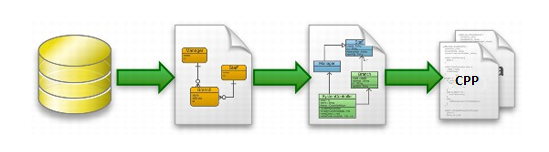
\includegraphics[width=1\textwidth]{images/orm.png}
		\caption{Uproszczony przebieg generowania opisu mapowania obiektowo-relacyjnego \cite{ormimg}.}
	\end{figure}

\subsection{Wzorzec projektowy}
	\indent Wzorce projektowe są obecnie szeroko stosowane przy tworzeniu oprogramowania. Pozwalają one na wyodrębnienie często używanych części algorytmów, tak aby mogły być używane przez różne części systemu. Nie są to gotowe rozwiązania, a jedynie opisy oraz szablony zawierające wskazówki rozwiązania tych samych problemów występujących w różnych sytuacjach. \\
	\indent Wzorce programowania obiektowego zazwyczaj pokazują relacje i powiązania pomiędzy obiektami bez specyfikacji tych obiektów. Są one stosowane na poziomie projektowania aplikacji. \\
	\indent Typy wzorców projektowych możemy podzielić na:
	\begin{itemize}
		\item{Wzorce konstrukcyjne - opisujące proces tworzenia nowych obiektów. Ich zadaniem jest tworzenie, inicjalizacja oraz konfiguracja obiektów.}
		\item{Wzorce strukturalne - opisujące struktury powiązanych ze sobą obiektów.}
		\item{Wzorce czynnościowe - opisujące zachowanie i powiązania współpracujących ze sobą obiektów.}
	 \end{itemize} 
\subsection{Wzorzec Model-Widok-Kontroler}
	\indent Wzorzec projektowy model-widok-kontroler oddziela od siebie warstwy: dostępu do danych, kontrolera oraz widoku. Każda warstwa odpowiada za inne zadania.
	\begin{itemize}
	\item Warstwa modelu - zarządza dostępem do danych oraz wszelkimi zmianami z nimi związanymi
	\item Warstwa kontrolera - interpretuje sygnały płynące z warstwy widoku. Informuje warstwy dostępu do danych oraz widoku o wymaganych zmianach.
	\item Warstwa widoku - zarządza wyświetlaniem informacji. 
	\end{itemize}
Przykładowy obrazek przedstawia w prosty sposób schemat działania tego wzorca oraz przepływ informacji między warstwami. \\
\begin{figure}[h]
	\centering
	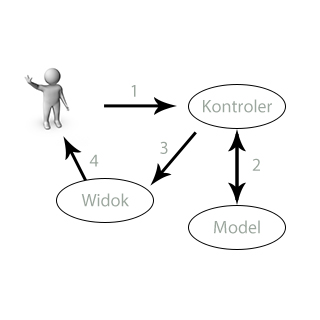
\includegraphics[width=0.6\textwidth]{images/mvc.jpg}
	\caption{Wzorzec Model-Widok-Kontroler. \cite{mvcimg}}
\end{figure}
\FloatBarrier
\subsection{Wzorzec DAO}
	\indent DAO jest komponentem, którego zadaniem jest dostarczanie jednolitego interfejsu do komunikacji między aplikacją, a źródłem danych(np. bazą danych czy plikiem). DAO dostarcza możliwość manipulacji danymi bez wykonywania bezpośrednich operacji na źródle danych, a jedynie na obiekcie. Głównymi zaletami takiego podejścia są prostota użycia i czytelność. Zmiana logiki nie wymaga zmian w źródle danych i na odwrót. Pozwala to również ukryć szczegóły związane ze źródłem danych oraz w łatwy sposób zmienić je w razie potrzeby \cite{dao}. \\
	\indent Wadami tego rozwiązania jest pojawienie się kolejnej warstwy interfejsu oraz zwiększenie ilości kodu, który musi zostać wykonany do realizacji dostępu do danych.
\begin{figure}[h]
	\centering
	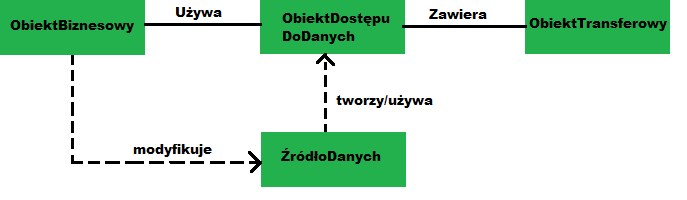
\includegraphics[width=0.8\textwidth]{images/dao.jpg}
	\caption{Wzorzec DAO \cite{daoimg}}
\end{figure}
\FloatBarrier
Jak widać w skład wzorca wchodzą:
\begin{itemize}
\item{Obiekct biznesowy(Business Object) - obiekt przechowujący dane biznesowe}
\item{Obiekt dostępu do danych(Data Access Object) - zapewnia transparentny dostęp do źródła danych}
\item{Źródło danych(Data Source) - baza danych, plik XML, itp.}
\item{Obiekt transferowy(Transfer Object) - przenosi dane z warstwy danych do obiektu biznesowego}
\end{itemize}
\subsection{Biblioteka współdzielona}
	\indent Biblioteka współdzielona jest ładowana tylko raz do pamięci systemu. Każdy proces który załaduje taka bibliotekę do własnej pamięci procesu jedynie mapuje adresy do oryginalnych wywołań funkcji. W przeciwieństwie do bibliotek statycznych kod funkcji nie jest kopiowany do pamięci procesu, który je wywołuje. Przechowywane są jedynie wirtualne adresy funkcji do których odwołuje się proces. Raz załadowana biblioteka współdzielona może być więc używana przez wiele procesów jednocześnie co zmniejsza zużycie pamięci \cite{dll}.
\begin{figure}[h]
	\centering
	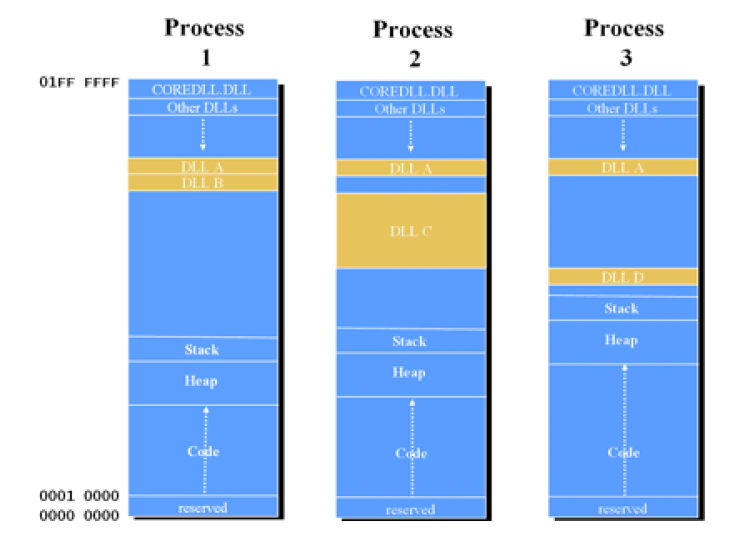
\includegraphics[width=0.7\textwidth]{images/dll.png}
	\caption{Schemat działania biblioteki współdzielonej \cite{dllimg}.}
\end{figure}
\FloatBarrier
\subsection{Qt framework}
	\indent Framework Qt jest gotowym narzędziem skierowanym do programistów C++, jak również osób preferujących język CSS i Javascript do budowania aplikacji. Posiada moduły potrzebne do budowy kompletnej aplikacji, m. in.:
	\begin{itemize}
	\item Biblioteki języka C++ przeznaczone na wiele platform
	\item Wsparcie dla budowania interfejsu użytkownika przy użyciu różnych narzędzie
	\item Zintegrowane środowisko deweloperskie
	\end{itemize}
	\indent Główną zaletą używania Qt jest możliwość pisania kodu skierowane pod wiele platform. Moduły obsługi bazy danych, budowy interfejsu użytkownika i wiele innych pozwalają znacznie skrócić czas potrzebny na tworzenie aplikacji. Jest również jednym z niewielu narzędzi w języku C++, które bardzo dobrze wspierają refleksję \cite{qtframework}.

\chapter{Analiza istniejących aplikacji do generowania opisu mapowania obiektowo-relacyjnego}\label{chap:analiza}
W tym rozdziale zostaną przeanalizowane istniejące aplikacje zajmujące się generowaniem opisu mapowania obiektowo-relacyjnego. Sprawdzone zostaną ich słabe i mocne stron oraz wymagania.
\section{Istniejące rozwiązania w dziedzinie}
\indent W języku C++ brak jest podobnych aplikacji zajmujących sie generowaniem warstwy dostępu do danych aplikacji. Istnieją aplikacje zajmujące się mapowaniem obiektowo-relacyjnym jednak bez funkcjonalności generowania jego opisu. W języku Java istnieje kilka aplikacji zajmujących się generowaniem opisu mapowania obiektowo-relacyjnego. Są nimi: JOOQ \cite{jooqweb} oraz Hibernate \cite{hibernateweb}. Obie aplikacje zajmują się mapowaniem obiektowo-relacyjnym i posiadają funkcjonalność generowania warstwy dostępu do danych z istniejących systemów relacyjnych baz danych.
\subsection{Wymagania aplikacji}
Obie aplikacje, tj. JOOQ oraz Hibernate zostały stworzone przy użyciu języka Java. Dzięki temu mogą one być używane zarówno na systemach unixowych jak i tych z rodziny Windows.
Sam Hibernate nie posiada opcji generowania modelu warstwy danych aplikacji. Dostępne są w tym celu odpowiednie wtyczki do środowisk programistycznych, takich jak Eclipse czy Intellij. Aplikacja JOOQ natomiast rozwiązała ten problem i udostępnia funkcję generatora kodu z linii poleceń wywołując odpowiednią klasę.
Jedynym wymogiem oprócz posiadania odpowiedniego środowiska z którego wygenerowany zostanie projekt na podstawie bazy danych jest stworzenie odpowiedniego pliku konfiguracyjnego.
\section{Wady i słabe punkty istniejących rozwiązań}
Jako pierwsze weźmy pod uwagę wady aplikacji Hibernate:
\begin{itemize}
\item{Bardzo duża ilość API\footnote{API(ang. Application Programming Interface) - dostarcza odpowiednie specyfikacje podprogramów, struktur danych, klas obiektów i wymaganych protokołów komunikacyjnych.}. do nauki, przez co nie jest łatwy w obsłudze.}
\item{Ze względu na budowę modelu warstwy danych aplikacji wymaga dużej ilości zapytań do bazy. Często przy bazach z dużą ilością rekordów wydajność zauważalnie spada.}
\item{Wymaga użycia odpowiedniego środowiska programistycznego i wtyczek w celu generowania warstwy dostępu do danych aplikacji.}
\end{itemize}

Druga aplikacja JOOQ rozwiązuje dwie z trzech wyżej wymienionych wad. Niestety nadal oferuje one generowanie modelu danych z zachowaniem czystego wzorca DAO, co wiąże się z większym zużyciem pamięci i w pewnych sytuacjach stratami wydajności. Oczywiście tego typu rozwiązania posiadają również bardzo wiele zalet:
	
\begin{itemize}
\item{Nie wymagają od programisty znajomości języka SQL.}
\item{Oszczędzają dużo czasu, ponieważ same zajmują się komunikacją z bazą i pozyskiwaniem danych.}
\item{Pozwalają skupić się na logice biznesowej aplikacji, zamiast zarządzaniu bazą danych.}
\item{Są niezależne od systemów baz danych. Mogą współpracować z wieloma róznymi systemami.}
\end{itemize}

Są to najważniejsze zalety tego typu rozwiązań. Jednak jeśli chodzi o analizowanie w tym rozdziale aplikacje, żadna z nich nie współpracuje z aplikacjami pisanymi w języku C++. Pozwala to zaproponować własne rozwiązanie i wypełnić tę lukę.
\chapter{Technologie i metody użyte w części badawczej}\label{chap:technologie}
W tym rozdziale zostaną opisane wszelkie użyte narzędzia oraz technologie, które posłużyły do stworzenia aplikacji Qubic. Zostanie opisany wybrany serwer bazy danych, a następnie środowisko deweloperskie. W dalszej części zostaną przedstawione użyte technologie wraz z metodykami programistycznymi użytymi w fazie projektowania aplikacji. 
\subsection{Język programowania}
Do stworzenia aplikacji został wybrany język C++. Najważniejszym czynnikiem jego wyboru jest wydajność. W porównaniu podstawowych operacji między innymi popularnymi językami język ten jest zdecydowanie szybszy. Poniższa tabela przedstawia porównanie czasów wykonania: pętli, operacji tablicowych, podstawowych operacji matematycznych.
\begin{figure}[h]
	\centering
	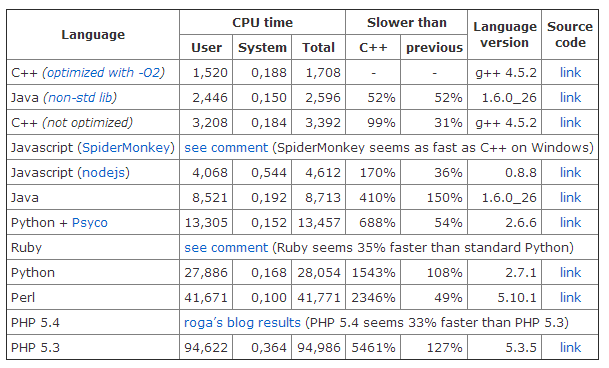
\includegraphics[width=1.1\textwidth]{images/c++test.png}
	\caption{Porównanie wydajności popularnych języków względem C++. \cite{c++testimg}}
\end{figure}
\FloatBarrier

Drugim ważnym czynnikiem wyboru języka C++ jest brak istnienia aplikacji realizujących mapowanie obiektowo-relacyjne wraz z możliwością generowania warstwy dostępu do danych w tym języku.

\subsection{System baz danych}
Jako system zarządzania bazą danych został wybrany serwer MySQL. Czynniki które o tym zdecydowały to przede wszystkim mała zajętość pamięci oraz łatwa i szybka konfiguracja. Dodatkowo posiada on bardzo dobrą integrację z użytym frameworkiem Qt, który został użyty m.in.: w celu połączenia z bazą danych oraz odczytu jej struktury z poziomu języka C++.
\subsection{Środowisko deweloperskie}
Wybrane środowisko deweloperskie jest częścią użytego frameworka Qt. Qt Creator jest zintegrowany z zestawem bibliotek użytego frameworka i udostępnia wsparcie składni oraz informacje o interfejsie programowania aplikacji.
\subsection{Biblioteki}
Użyty zestaw bibliotek należy do frameworka Qt. Udostępnia on biblioteki przenośne i narzędzia programistyczne dedykowane dla języków C++, Java czy QML. Głównym atutem są klasy służące do budowy graficznego interfejsu użytkownika, wsparcie połączenia z wieloma systemami baz danych oraz obsługiwany mechanizm refleksji. Wszystkie te rzeczy w znacznym stopniu ułatwiają tworzenie aplikacji oraz skracają czas potrzebny na jej stworzenie.
\subsection{Inne narzędzia}
Dodatkowym narzędziem użytym w procesie tworzenia aplikacji był system kontroli wersji o nazwie GIT. Pozwalało to kontrolować cały proces powstawania Qubica. Całość jest zintegrowana z portalem Github i przechowywana na prywatnym repozytorium.

\begin{figure}[h]
	\centering
	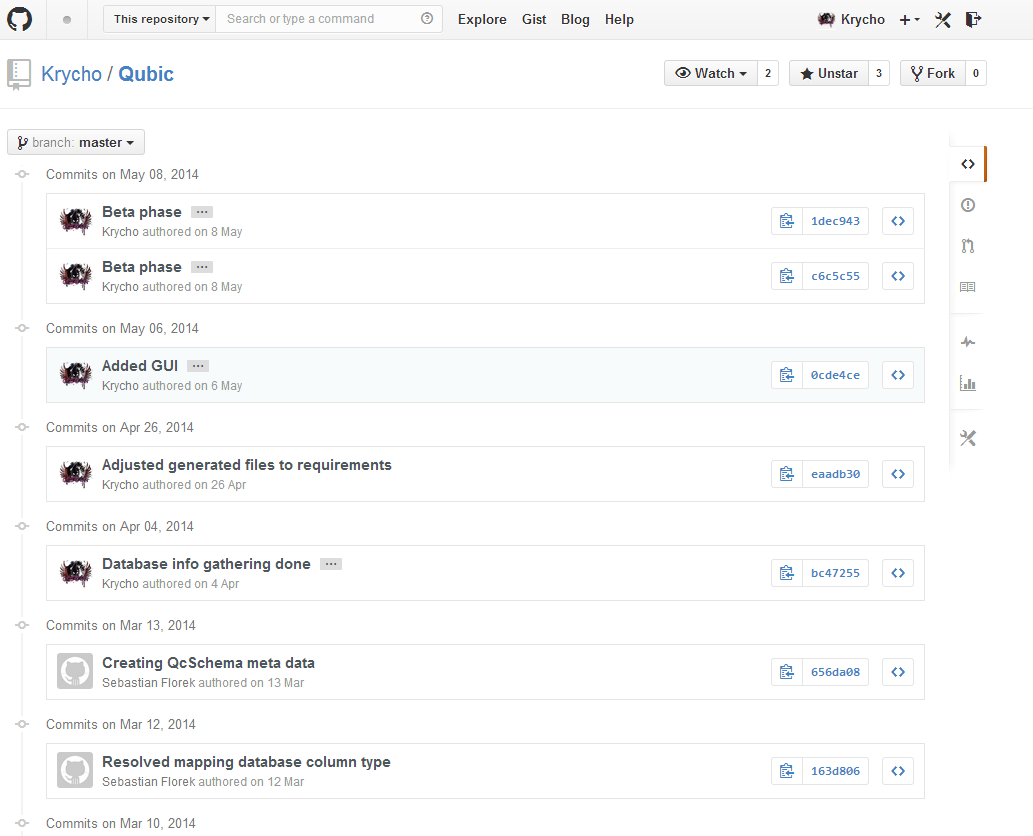
\includegraphics[width=.9\textwidth]{images/git.png}
	\caption{Log kontrolny zmian projektowych z portalu Github.}
\end{figure}
\FloatBarrier

\chapter{Projektowanie aplikacji szkieletowej Qubic} \label{rozdz.czesc.prakt}

\section{Analiza wymagań}
	\indent W tym rozdziale zostanie przedstawiona analiza oraz część implementacyjna aplikacji Qubic. W pierwszej części są zdefiniowane wymagania aplikacji oraz opisane wymagania funkcjonalne wraz z ograniczenia projektu. Następnie zostają przedstawione główne diagramy dotyczące działania aplikacji. Kolejna część opisuje technologie i metodologie użyte w projekcie z podziałem na warstwy modelu, widoku i kontrolera w aplikacji. Kolejna część zawiera przedstawienie proponowanego rozwiązania wraz z częścią implementacyjna. Przybliżone zostają najważniejsze części kodu wraz z opisem. Ostatnim krokiem są testy i ocena funkcjonalności stworzonej aplikacji.
\subsection{Studium możliwości}
	\indent Główną ideą projektu jest rozwiązanie problemu generowania warstwy dostępu do danych aplikacji. W celu minimalizacji zużycia pamięci oraz uzyskania jak najlepszej wydajności została stworzona jedna warstwa obiektów, gdzie każdy obiekt klasy odzwierciedla tabelę w bazie danych. Nie istnieje podział na obiekty transakcyjne i biznesowe. Aplikacja daje nam możliwość generowania warstwy dostępu do danych z większości obecnie istniejących systemów zarządzania relacyjnymi bazami danych.
\subsection{Wymagania funkcjonalne}
	\indent Ze względu na budowę własnego systemu mapowania obiektowo-relacyjnego moduł generowania danych musi spełniać pewne wymagania:
	\begin{enumerate}
	\item{Generowanie warstwy dostępu do danych w oparciu o relacyjne bazy danych.}
	\item{Generowanie plików klas oraz plików źródłowych.}
	\item{Generowane pliki powinny mieć czytelną i prostą budowę, aby były proste w użyciu dla programistów.}
	\item{Aplikacja powinna trzymać dane struktury bazy w pamięci podręcznej w celu zachowania wydajności i zlikwidowania problemu częstego dostępu do bazy danych.}
	\item{Wszelkie ustawienia powinny być w prosty sposób konfigurowalne, tak by zmiana w bazie nie wymuszała zmian kodu aplikacji.}
	\item{Powinna generować dodatkowe funkcje pozwalające wyciągnąć powiązane dane w oparciu o relacje między tabelami.}
	\item{Aplikacja powinna wspierać wiele systemów baz danych lub udostępniać łatwy sposób dodania ich wsparcia.}
	\item{Aplikacja powinna w prosty sposób definiować mapowanie typów danych z bazy danych na typy języka.}
	\end{enumerate}
\subsection{Ograniczenia projektu}
	\indent Ze względu na czytelność kodu oraz sposób działania modułu zajmującego się mapowanie obiektowo-relacyjnym na bazę danych zostały nałożone pewne ograniczenia:
	\begin{itemize}
	\item{Każda tabela w bazie musi zawierać klucz główny.}
	\item{Każdy typ danych użyty w bazie musi zostać zarejestrowany w aplikacji i zmapowany na odpowiedni typ języka.}
	\item{Nazwy kolumn w tabelach mogą zawierać jedynie litery i cyfry ze względu na czytelność generowanego kodu.}
	\end{itemize}
	\indent Powyższe ograniczenia są rozpoznawane przez aplikację, a ich nie spełnienie wiąże się z brakiem możliwości generowania warstwy dostępu do danych. Kolejnym ograniczeniem jest brak integracji generatora z innymi aplikacjami do mapowania obiektowo-relacyjnego oraz współpraca jedynie z relacyjnymi bazami danych. Również błędne wskazanie relacji w tabelach może wiązać się z błędami logicznymi w wygenerowanym kodzie.
\section{Projekt}
\subsection{Projekt warstwy danych}\label{sec:database}
\indent Poniżej przedstawiony kod został użyty do budowy bazy danych. Baza zawiera najważniejsze relacje potrzebne do testów tworzonej aplikacji, tj. jeden do wielu oraz wiele do wielu.
\begin{framed}
\lstinputlisting[language=SQL]{additional/database.sql}
\end{framed}

Użytkownik bazy danych, który posłuży nam do ustanowienia połączenia musi posiadać uprawnienia do odczytu informacji z tabel opisujących budowę bazy danych. Przykładowo baza MySQL posiada dodatkową bazę przechowująca informacje o strukturze danych w systemie. Zaleca się więc używanie konta administratora bazy w celu generowania plików warstwy danych.\\
\indent Poniższy rysunek przedstawia stworzoną bazę danych w postaci graficznej wraz z zaznaczeniem relacji między tabelami.
\subsection{Projekt aplikacji}
	\indent Projektowana aplikacja została oparta o wzorzec model-widok-kontroler, gdzie modelem jest baza danych, kontrolerem biblioteka współdzielona, natomiast widokiem przykładowa aplikacja korzystająca z funkcji udostępnianych przez bibliotekę. Poniższy diagram przypadków użycia przedstawia możliwości generatora:

\begin{figure}[h]
	\centering
	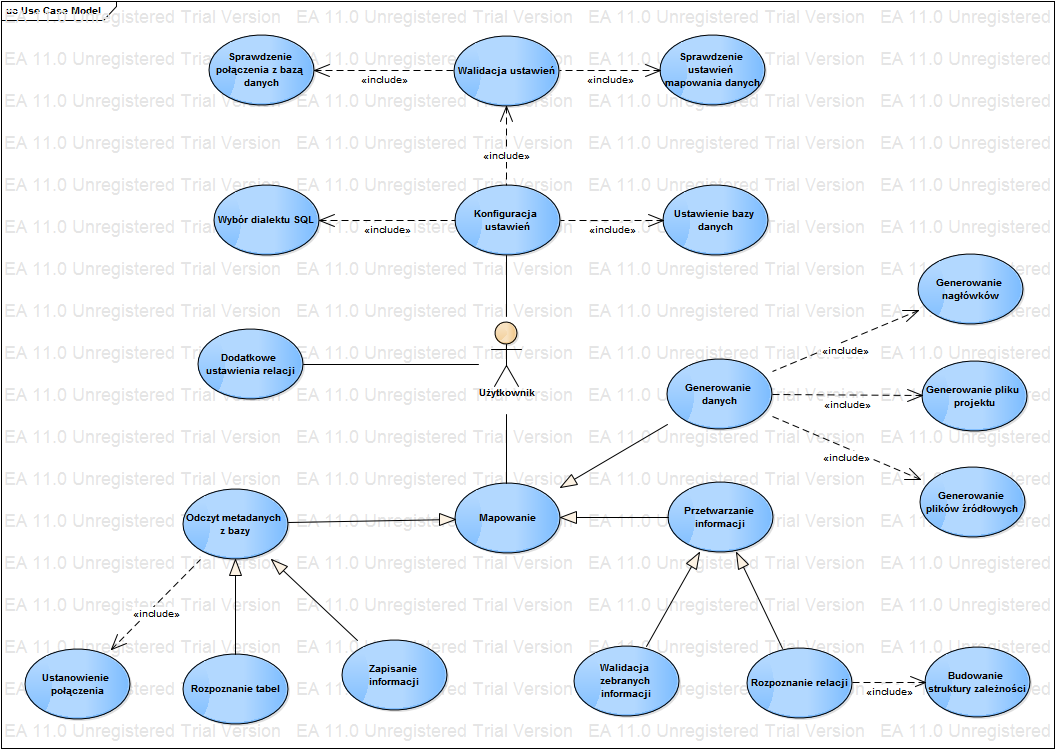
\includegraphics[width=1.5\textwidth, angle=90]{images/QubicUseCase.png}
	\caption{Diagram przypadków użycia modułu generatora.}
\end{figure}
\FloatBarrier

Użytkownik ma możliwość konfiguracji ustawień aplikacji. Wszystkie ustawienia są sprawdzane przed połączeniem z bazą danych. Kolejną rzeczą jest opcja ręcznego definiowania relacji wiele do wielu między tabelami. Inne rodzaje relacji są rozpoznawane automatycznie. Ostatnim krokiem jest złożony proces mapowania, który najpierw odczytuje dane z bazy i zapisuje je do pamięci, następnie przeprowadza walidacje zebranych informacji oraz buduje struktury zależności. Ostatnim krokiem jest sam proces generowania projektu gotowego użycia w środowisku programistycznym. \\
	\indent Poniższy diagram koncepcyjny przedstawia strukturę aplikacji:
	
\begin{figure}[h]
	\centering
	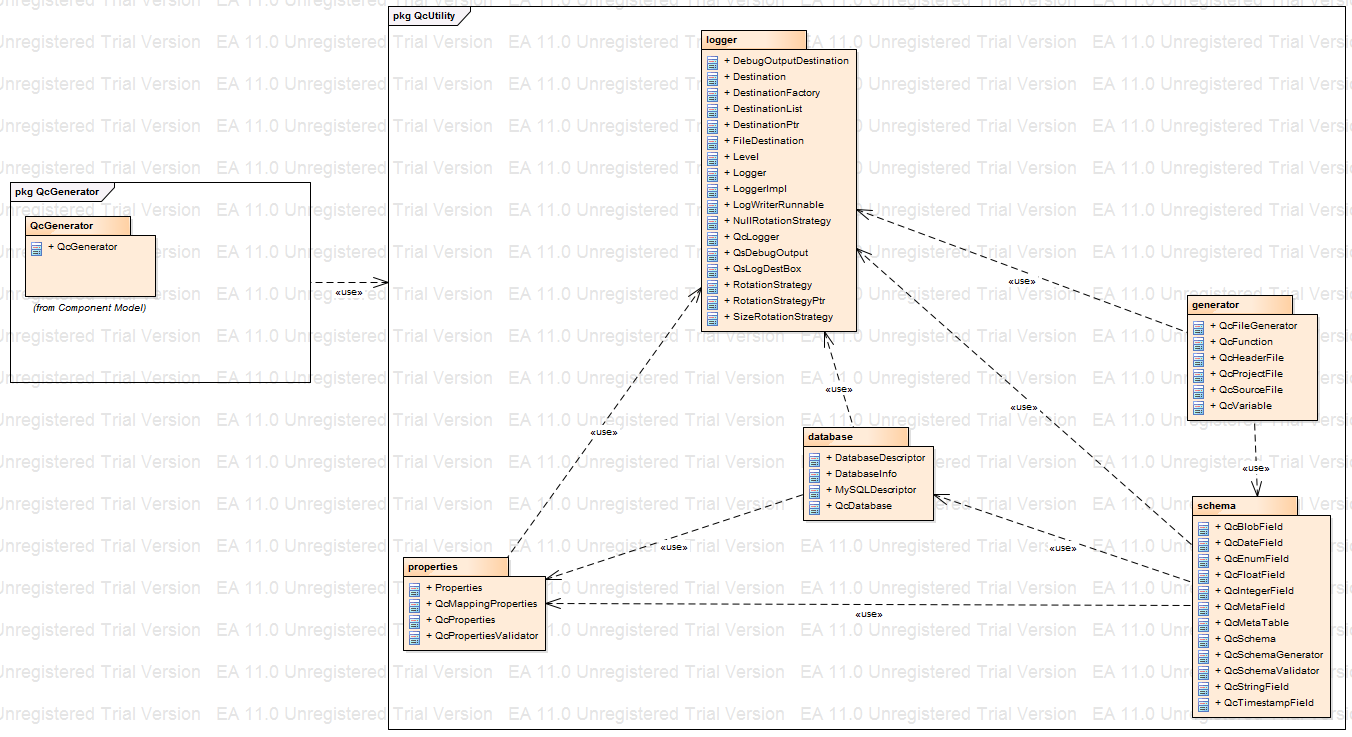
\includegraphics[width=1.6\textwidth, angle=90]{images/Qubic.png}
	\caption{Diagram koncepcyjny generatora.}
\end{figure}
\FloatBarrier

Paczka QcUtility jest w istocie biblioteką współdzieloną realizującą generowanie opisu mapowania obiektowo-relacyjnego. Moduł QcGenerator natomiast jest aplikacją opartą o funkcjonalność udostępnioną przez bibliotekę. Warstwą modelu danych jest baza danych, której struktura została przedstawiona we wcześniejszym rozdziale. Nie jest ona częścią samej aplikacji, dlatego nie została przedstawiona na diagramie. \\
	\indent Moduł główny zajmujący się generowaniem został podzielony na logiczne części w celu wyraźnej separacji odpowiedzialności każdego modułu\footnote{Zasada pojedynczej odpowiedzialności mówi że procesy powinny być od siebie niezależne i zaimplementowane w postaci oddzielnych klas lub modułów, które komunikują się ze sobą przy pomocy publicznych interfejsów.}.

\begin{figure}[h]
	\centering
	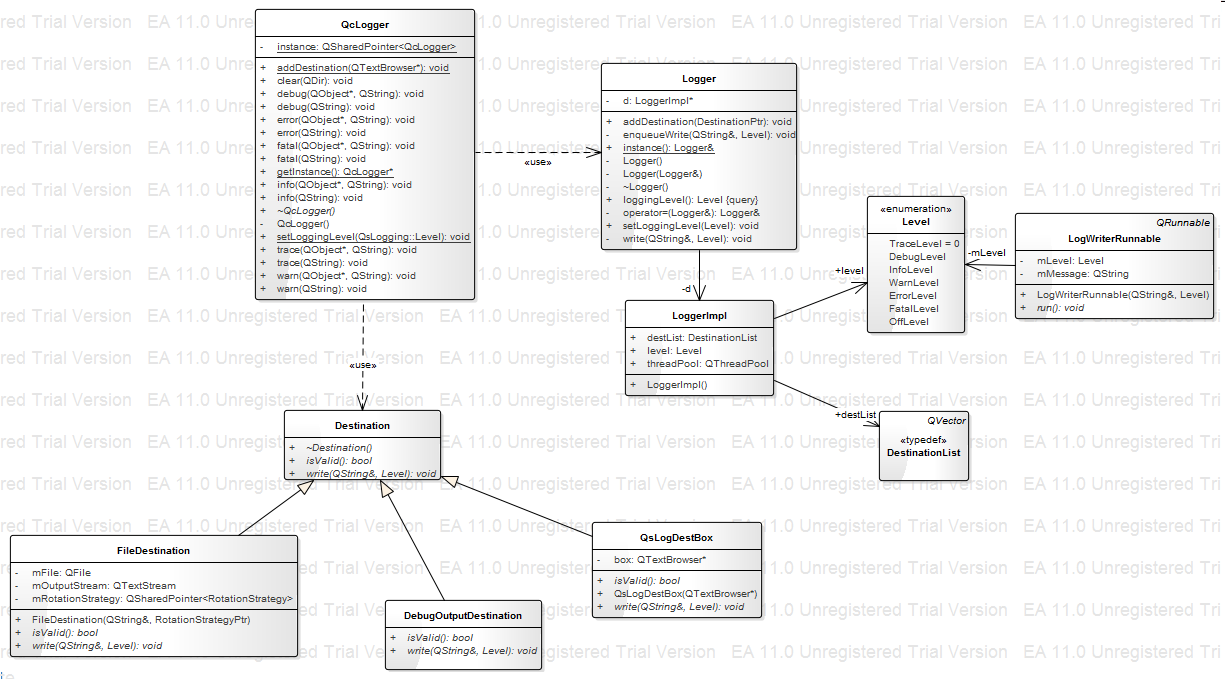
\includegraphics[width=.95\textwidth, angle=90]{images/logger.png}
	\caption{Diagram klas modułu logera.}
\end{figure}
\FloatBarrier

Moduł logujący jest używany przez wszystkie inne części systemu. Pozwala on w prosty i przejrzysty sposób śledzić przebieg procesu mapowania oraz wychwycić ewentualne błędy. Oparty on został o istniejący projekt logera o nazwie QsLog. 

\begin{figure}[h]
	\centering
	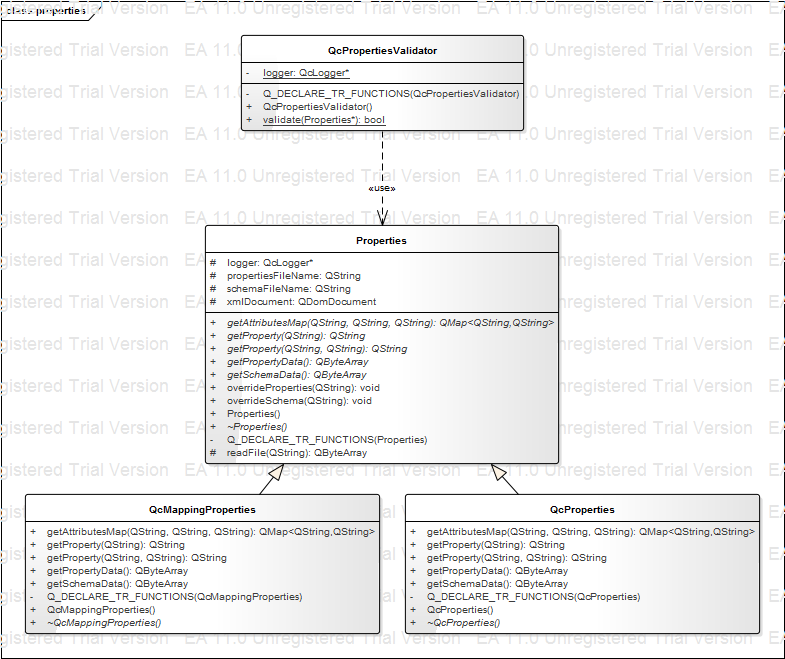
\includegraphics[width=1.1\textwidth]{images/properties.png}
	\caption{Diagram klas modułu ustawień.}
\end{figure}
\FloatBarrier	

Wszelkie ustawienia potrzebne do połączenia z bazą danych oraz do przeprowadzenia procesu mapowania tabel na klasy są obsługiwane przez powyższy moduł. Udostępniony został również interfejs sprawdzający poprawność ustawień.

\begin{figure}[h]
	\centering
	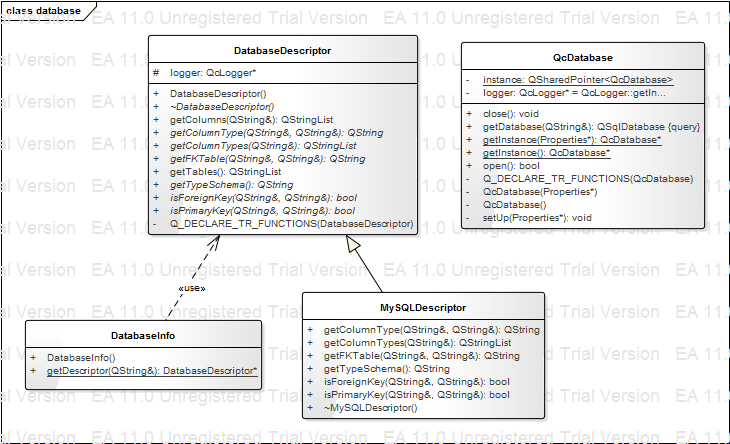
\includegraphics[width=1.1\textwidth]{images/database.png}
	\caption{Diagram klas modułu ustawień.}
\end{figure}
\FloatBarrier	

Moduł bazy danych pełni kilka funkcji:
\begin{itemize}
\item{jest odpowiedzialny za utworzenie połączenia z bazą danych i odczyt metadanych z bazy}
\item{zbiera informacje o nazwach tabelach, typach danych w tabelach, kluczach głównych, kluczach obcych oraz powiązanych tabelach i przekazuje je do modułu zajmującego się przetwarzaniem tych informacji.}
\end{itemize}

\begin{figure}[h]
	\centering
	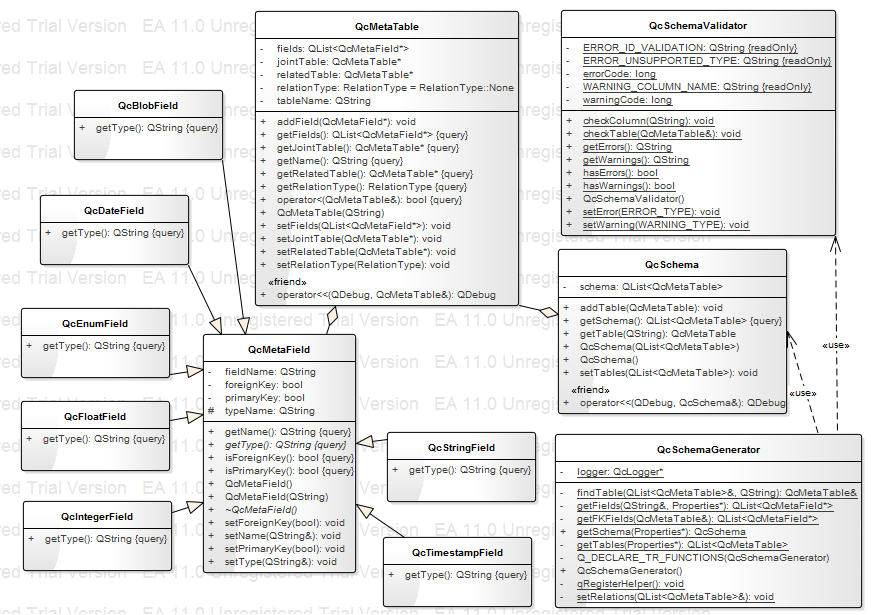
\includegraphics[width=1.1\textwidth]{images/schema.png}
	\caption{Diagram klas modułu budowania struktury danych.}
\end{figure}
\FloatBarrier	

Powyższy moduł jest najważniejszą częścią aplikacji. Jego zadaniem jest przetworzenie zebranych informacji.
\begin{itemize}
\item{tworzy w pamięci strukturę odczytanych tabel}
\item{automatycznie rozpoznaje relacje między tabelami(jeden do jednego, jeden do wielu)}
\item{mapuje typy kolumn bazy danych na odpowiednie typy języka}
\item{sprawdza czy zebrane dane spełniają postawione założenia}
\item{udostępnia interfejs generujący}
\end{itemize}

\begin{figure}[h]
	\centering
	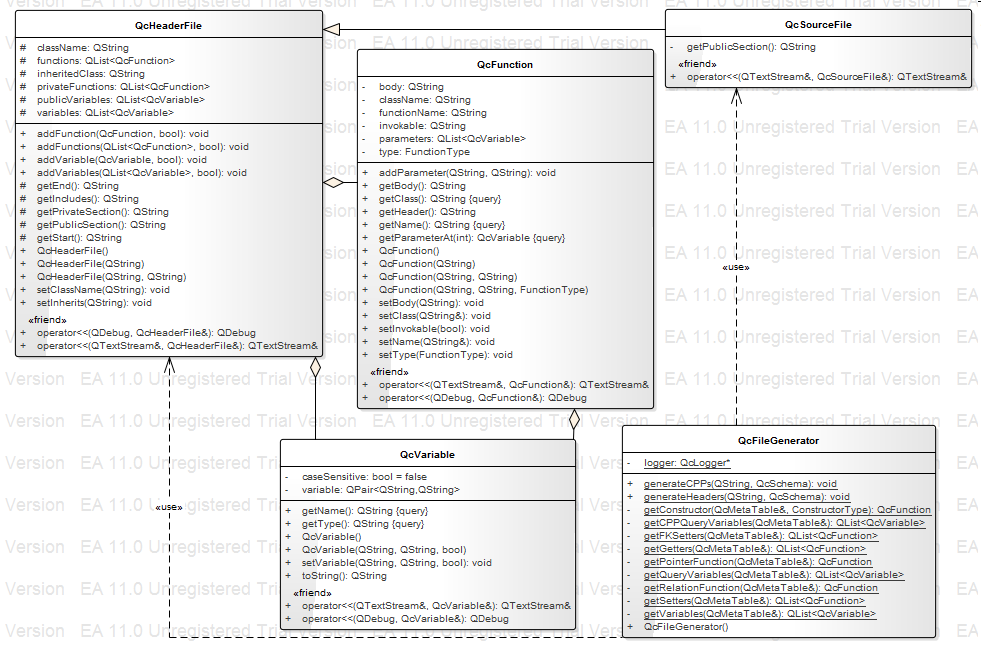
\includegraphics[width=1.1\textwidth]{images/generator.png}
	\caption{Diagram klas modułu generatora projektu.}
\end{figure}
\FloatBarrier	

Ostatni moduł udostępnia generator plików, który bazując na wygenerowanej strukturze danych tworzy gotowy projekt dla programisty. Wszystkie zebrane informacje są przekształcane w gotowe pliki nagłówkowe i źródłowe języka C++.

\section{Implementacja: punkty kluczowe}
W tej części pracy zostaną przedstawione kluczowe fragmenty kodu odpowiadające ze główny przepływ danych przy generowaniu opisu mapowania obiektowo-relacyjnego. Główny moduł biblioteki współdzielonej oraz przykładowa aplikacja z interfejsem graficznym wykorzystująca udostępniane przez stworzoną bibliotekę funkcje. \\
	\indent Do połączenia z bazą została użyta klasa zaprojektowana zgodnie z wzorcem projektowym o nazwie singletone\footnote{Singletone - wzorzec projektowy ograniczający możliwość tworzenia obiektów danej klasy do jednej instancji oraz zapewniający globalny dostęp do stworzonego obiektu.}.
	
\begin{framed}
\lstinputcplusplus[caption={QcDatabase}]{additional/qcdatabase.h}
\end{framed}

Kolejna klasa udostępnia interfejs zajmujący się odczytywaniem metadanych z bazy. Została tutaj użyta klasa abstrakcyjna w celu umożliwienia łatwego dodania wsparcia nowych dialektów SQL.

\begin{framed}
\lstinputcplusplus[caption={QcDatabase}]{additional/databasedescriptor.h}
\end{framed}

Przykładowa implementacja takiej klasy dla dialektu MySQL widoczna jest poniżej.

\begin{framed}
\lstinputcplusplus[caption={QcDatabase}]{additional/mysqldescriptor.cpp}
\end{framed}

Poniższa klasa QcMetaField jest odpowiednikiem kolumny w tabeli i przechowuje informacje o jej typie oraz właściwościach, np. czy jest kluczem głównym. Jest to również klasa abstrakcyjna i w celu zarejestrowania nowego typu, który będzie obsługiwany przez aplikację należy rozszerzyć tą klasę, dodać wpis do funkcji w klasie QcSchemaGenerator w celu zarejestrowania klasy w systemie refleksji Qt oraz zarejestrować nowy typ w odpowiednim pliku z ustawieniami mapowania danych.

\begin{framed}
\lstinputcplusplus[caption={QcDatabase}]{additional/qcmetafield.h}
\end{framed}

Jedna z najważniejszych klas modułu generatora to klasa QcSchemaGenerator, która zajmuje się przetworzeniem informacji pobranych z bazy danych na odpowiednią strukturę danych przechowywaną w pamięci. Główna funkcja getTables jest odpowiedzialna za odczytanie tabel, nazw i typów kolumn oraz rozpoznanie części relacji między tabelami. W trakcie przetwarzania wykonywana jest również walidacja danych.

\begin{framed}
\lstinputcplusplus[caption={QcDatabase}]{additional/qcschemagenerator.cpp}
\end{framed}

Na podstawie utworzonej struktury danych generowane są pliki projektu. Odpowiada za to klasa QcFileGenerator.

\begin{framed}
\lstinputcplusplus[caption={QcDatabase}]{additional/qcfilegenerator.h}
\end{framed}

Poniżej przedstawiony jest częściowy kod prostej aplikacji graficznej opartej o funkcje udostępniane przez stworzoną bibliotekę. Odczytuje ona odpowiednie pliki ustawień, łączy się z bazą danych, sprawdza ustawienia, a następnie generuje projekt wykorzystywany przez moduł mapowania obiektowo-relacyjnego.

\begin{framed}
\lstinputcplusplus[caption={QcDatabase}]{additional/qcgenerator.cpp}
\end{framed}

\section{Testy stworzonej aplikacji}
\subsection{Testy wydajności}
Test wydajności został przeprowadzony w porównaniu z aplikacją JOOQ napisaną w języku Java. Porównany został czas potrzebny na wygenerowanie plików gotowego projektu. Użyta została baza danych opisana w rozdziale \ref{sec:database}. Oto logi przebiegu procesu generowania wraz z czasami.

\begin{framed}
\lstinputlisting[caption={JOOQ Log}]{additional/jooq.log}
\end{framed}

\begin{figure}[h]
	\centering
	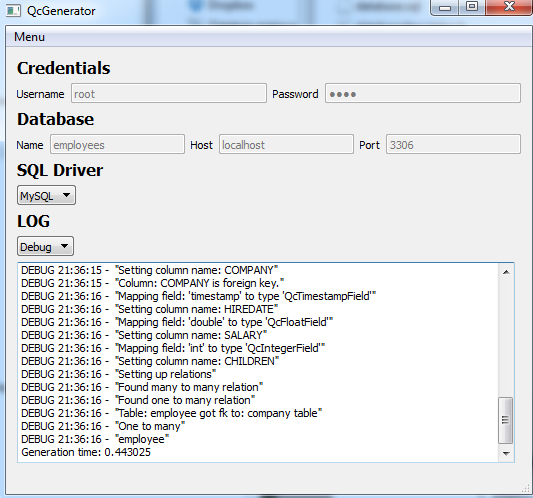
\includegraphics[width=1.1\textwidth]{images/qubic-gen.png}
	\caption{Interfejs aplikacji przykładowej wraz z logiem procesu generowania.}
\end{figure}
\FloatBarrier

\begin{table}[!ht]
\centering
    \begin{tabular}{cccc}
    \hline
    Framework & Czas generowania & Poprawa wydajności(w \%) \\ \hline
    Qubic & 443.025 ms &  - \\ \hline
    JOOQ & 681.673 ms & 35 \\ \hline
    \end{tabular}
    \caption{Porównanie czasów generowania projektu z istniejącej bazy danych.}
\end{table}

\subsection{Porównanie funkcjonalności}  

Porównanie funkcjonalności samego generatora opisu mapowania obiektowo-relacyjnego opiera się na sprawdzeniu wsparcia różnych dialektów SQL. Porównane zostały jedynie najpopularniejsze dialekty.
\begin{table}[!ht]
\centering
    \begin{tabular}{ccccc}
    \hline
    Framework & Qubic & JOOQ & Hibernate & Funkcjonalność \\ \hline
    & tak & tak & tak & Wsparcie MySQL \\ \hline
& tak & tak & tak & Wsparcie PostgreSQL \\ \hline
& tak & tak & nie & Wsparcie SQLite \\ \hline
& tak & tak & tak & Wsparcie Oracle \\ \hline
& tak & nie & tak & Wsparcie MSSQL \\ \hline
& tak & tak & tak & Wsparcie Sybase \\ \hline
& tak & tak & tak & Wsparcie IBM DB2 \\ \hline
    \end{tabular}
    \caption{Porównanie funkcjonalności wybranych aplikacji zajmujących się generowaniem opisu mapowania obiektowo-relacyjnego.}
\end{table}

\chapter{Podsumowanie}
Ten rozdział zawiera podsumowanie pracy oraz uzyskanych wyników. Omówione zostają dodatkowe możliwości rozwoju tematu jak i całej aplikacji Qubic.
\section{Dyskusja wyników}
Przeprowadzone testy generowania warstwy dostępu do danych aplikacji wykazały około 35\% wzrost wydajności na korzyść zaproponowanego rozwiązania. Należy tu zaznaczyć, że w języku C++ nie znaleziono podobnych aplikacji, a różnice wydajności wynikają częściowo z budowy języka Java, w którym zostały napisane podobne aplikacje. Dodatkowym atutem stworzonej aplikacji jest wsparcie większej ilości dialektów SQL od konkurencyjnych rozwiązań oraz brak istnienia podobnych aplikacji w języku C++, dzięki czemu Qubic staje się bezkonkurencyjnym rozwiązanie w swojej dziedzinie. Prostota użycia, brak zależności od zewnętrznych aplikacji czy dodatkowego ręcznego konfigurowania to tylko kilka z wielu atutów stworzonego generatora opisu mapowania obiektowo-relacyjnego.
\section{Ocena możliwości wdrożenia Qubica}
Qubic pozwala zaoszczędzić programistom dużą ilość czasu w fazie tworzenia aplikacji, dzięki czemu mogą sie oni skupić na innych częściach projektu. Moduł generujący warstwę dostępu do danych jest prosty i szybki w użyciu oraz dalszym rozwoju. W razie potrzeby jest prosto konfigurowalny, a dzięki generycznej budowie aplikacja może być łatwo dostosowywana do własnych potrzeb. Dzięki temu jej wdrożenie nie wiąże się z dużymi kosztami, a pozwala na późniejsze zaoszczędzenie cennego czasu w fazie implementacyjnej.
\section{Perspektywy dalszego rozwoju}
Dodatkowym atutem stworzonej aplikacji byłby moduł zajmujący się procesem odwrotnym, czyli generowaniem bazy danych z istniejącego schematu obiektów klas lub pliku tworzącego bazę danych. Pozwoliło by to na pewną swobodę programistom, których zadaniem jest stworzenie bazy, a łatwiejsze jest dla nich stworzenie struktury w języku programowania niż bezpośrednie tworzenie bazy danych używając język SQL.
\addcontentsline{toc}{chapter}{Bibliografia} 
\begin{thebibliography}{99}
	\bibitem{ejb} {M. Keith, M. Schincariol, Pro EJB 3 Java persistence API. 2006. ISBN-13 978-1-59059-645-6}
	\bibitem{hibernateInAction} {C. Bauer, G. King, Hibernate w akcji, 2007, ISBN: 978-83-246-0527-9}
	\bibitem{c++patterns} {A. Ezust, P. Ezust, Introduction to Design Patterns in C++ with Qt ISBN 978-0-13-282645-7}
	\bibitem{c++2} {D. Gennaro Advanced C++ Metaprogramming ISBN-13 978-1460966167}
	\bibitem{sql} {P. Wilton, J. Colby, Beginning SQL ISBN 0-7645-7732-8}
	\bibitem{mysqlweb} {http://dev.mysql.com/doc/refman/5.6/en/ - [dostęp 05.08.2014]}
	\bibitem{strostrup} {http://www.stroustrup.com/C++11FAQ.html - [dostęp 10.08.2014]}
	\bibitem{qtframework} {http://qt-project.org/ - [dostęp 07.01.2014]}
	\bibitem{dll} {http://msdn.microsoft.com/en-us/library/windows/desktop/ms681914(v=vs.85).aspx - [dostęp 29.07.2014]}
	\bibitem{hibernateweb} {http://docs.jboss.org/hibernate/orm/4.3/manual/en-US/html/ - [dostęp 02.08.2014]}
	\bibitem{jooqweb} {http://www.jooq.org/javadoc/3.4.x/ - [dostęp 02.08.2014]}
	%wzorce
	\bibitem{mvc} {http://msdn.microsoft.com/en-us/library/ff649643.aspx - [dostęp 28.07.2014]}
	\bibitem{dao} {http://www.oracle.com/technetwork/java/dataaccessobject-138824.html - [dostęp 28.07.2014]}
	\bibitem{datalayer} {http://msdn.microsoft.com/en-us/library/ee658127.aspx - [dostęp 27.07.2014]}
	%obrazki
	\bibitem{ormimg} http://www.visual-paradigm.com/VPGallery/img/orm/Overview/ORM-Overview.png --  [dostęp 02.11.2013]
	\bibitem{c++testimg} http://blog.famzah.net/2010/07/01/cpp-vs-python-vs-perl-vs-php-performance-benchmark/ - [dostęp 02.07.2014]
	\bibitem{mvcimg} {http://webroad.pl/wp-content/uploads/2012/12/images\_old\_mvs-schemat.jpg - [dostęp 28.07.2014]}
	\bibitem{daoimg} {http://www.oracle.com/ocom/groups/public/@otn/documents/digitalasset/146804.jpg - [dostęp 28.07.2014]}
	\bibitem{dllimg} {http://i.msdn.microsoft.com/dynimg/IC34006.gif - [dostęp 29.07.2014]}
\end{thebibliography}

\addcontentsline{toc}{chapter}{Spis rysunków} 
\listoffigures

\addcontentsline{toc}{chapter}{Spis tabel} 
\listoftables

\end{document}
